\documentclass[border=10pt]{standalone}
\usepackage{pgfplots}
\usepgfplotslibrary{colormaps}
\pgfplotsset{compat=1.18}
\begin{document}
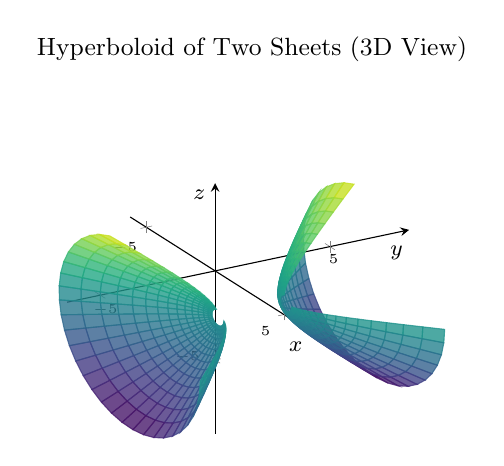
\begin{tikzpicture}
\begin{axis}[
    view={60}{30},
    xlabel={$x$}, ylabel={$y$}, zlabel={$z$},
    title={Hyperboloid of Two Sheets (3D View)},
    domain=0:360,
    y domain=0.3:2,
    samples=30,
    samples y=15,
    colormap/viridis,
    axis lines=center,
    enlargelimits=0.2,
    tick label style={font=\tiny},
    label style={font=\footnotesize},
    title style={font=\small},
    xlabel style={at={(ticklabel* cs:1)}, anchor=near ticklabel},
    ylabel style={at={(ticklabel* cs:1)}, anchor=near ticklabel},
    zlabel style={at={(ticklabel* cs:1)}, anchor=near ticklabel}
]
% Upper sheet: y = 1 + sqrt(2)*cosh(v), x = 1 + sqrt(2)*sinh(v)*cos(theta), z = -2 + sqrt(2)*sinh(v)*sin(theta)
\addplot3[surf, shader=flat corner, opacity=0.8] (
    {1 + sqrt(2)*sinh(y)*cos(deg(x))},
    {1 + sqrt(2)*cosh(y)},
    {-2 + sqrt(2)*sinh(y)*sin(deg(x))}
);

% Lower sheet
\addplot3[surf, shader=flat corner, opacity=0.8] (
    {1 + sqrt(2)*sinh(y)*cos(deg(x))},
    {1 - sqrt(2)*cosh(y)},
    {-2 + sqrt(2)*sinh(y)*sin(deg(x))}
);
\end{axis}
\end{tikzpicture}
\end{document}
